% Options for packages loaded elsewhere
\PassOptionsToPackage{unicode}{hyperref}
\PassOptionsToPackage{hyphens}{url}
\PassOptionsToPackage{dvipsnames,svgnames,x11names}{xcolor}
%
\documentclass[
  letterpaper,
  DIV=11,
  numbers=noendperiod]{scrartcl}

\usepackage{amsmath,amssymb}
\usepackage{iftex}
\ifPDFTeX
  \usepackage[T1]{fontenc}
  \usepackage[utf8]{inputenc}
  \usepackage{textcomp} % provide euro and other symbols
\else % if luatex or xetex
  \usepackage{unicode-math}
  \defaultfontfeatures{Scale=MatchLowercase}
  \defaultfontfeatures[\rmfamily]{Ligatures=TeX,Scale=1}
\fi
\usepackage{lmodern}
\ifPDFTeX\else  
    % xetex/luatex font selection
\fi
% Use upquote if available, for straight quotes in verbatim environments
\IfFileExists{upquote.sty}{\usepackage{upquote}}{}
\IfFileExists{microtype.sty}{% use microtype if available
  \usepackage[]{microtype}
  \UseMicrotypeSet[protrusion]{basicmath} % disable protrusion for tt fonts
}{}
\makeatletter
\@ifundefined{KOMAClassName}{% if non-KOMA class
  \IfFileExists{parskip.sty}{%
    \usepackage{parskip}
  }{% else
    \setlength{\parindent}{0pt}
    \setlength{\parskip}{6pt plus 2pt minus 1pt}}
}{% if KOMA class
  \KOMAoptions{parskip=half}}
\makeatother
\usepackage{xcolor}
\setlength{\emergencystretch}{3em} % prevent overfull lines
\setcounter{secnumdepth}{5}
% Make \paragraph and \subparagraph free-standing
\ifx\paragraph\undefined\else
  \let\oldparagraph\paragraph
  \renewcommand{\paragraph}[1]{\oldparagraph{#1}\mbox{}}
\fi
\ifx\subparagraph\undefined\else
  \let\oldsubparagraph\subparagraph
  \renewcommand{\subparagraph}[1]{\oldsubparagraph{#1}\mbox{}}
\fi

\usepackage{color}
\usepackage{fancyvrb}
\newcommand{\VerbBar}{|}
\newcommand{\VERB}{\Verb[commandchars=\\\{\}]}
\DefineVerbatimEnvironment{Highlighting}{Verbatim}{commandchars=\\\{\}}
% Add ',fontsize=\small' for more characters per line
\usepackage{framed}
\definecolor{shadecolor}{RGB}{241,243,245}
\newenvironment{Shaded}{\begin{snugshade}}{\end{snugshade}}
\newcommand{\AlertTok}[1]{\textcolor[rgb]{0.68,0.00,0.00}{#1}}
\newcommand{\AnnotationTok}[1]{\textcolor[rgb]{0.37,0.37,0.37}{#1}}
\newcommand{\AttributeTok}[1]{\textcolor[rgb]{0.40,0.45,0.13}{#1}}
\newcommand{\BaseNTok}[1]{\textcolor[rgb]{0.68,0.00,0.00}{#1}}
\newcommand{\BuiltInTok}[1]{\textcolor[rgb]{0.00,0.23,0.31}{#1}}
\newcommand{\CharTok}[1]{\textcolor[rgb]{0.13,0.47,0.30}{#1}}
\newcommand{\CommentTok}[1]{\textcolor[rgb]{0.37,0.37,0.37}{#1}}
\newcommand{\CommentVarTok}[1]{\textcolor[rgb]{0.37,0.37,0.37}{\textit{#1}}}
\newcommand{\ConstantTok}[1]{\textcolor[rgb]{0.56,0.35,0.01}{#1}}
\newcommand{\ControlFlowTok}[1]{\textcolor[rgb]{0.00,0.23,0.31}{#1}}
\newcommand{\DataTypeTok}[1]{\textcolor[rgb]{0.68,0.00,0.00}{#1}}
\newcommand{\DecValTok}[1]{\textcolor[rgb]{0.68,0.00,0.00}{#1}}
\newcommand{\DocumentationTok}[1]{\textcolor[rgb]{0.37,0.37,0.37}{\textit{#1}}}
\newcommand{\ErrorTok}[1]{\textcolor[rgb]{0.68,0.00,0.00}{#1}}
\newcommand{\ExtensionTok}[1]{\textcolor[rgb]{0.00,0.23,0.31}{#1}}
\newcommand{\FloatTok}[1]{\textcolor[rgb]{0.68,0.00,0.00}{#1}}
\newcommand{\FunctionTok}[1]{\textcolor[rgb]{0.28,0.35,0.67}{#1}}
\newcommand{\ImportTok}[1]{\textcolor[rgb]{0.00,0.46,0.62}{#1}}
\newcommand{\InformationTok}[1]{\textcolor[rgb]{0.37,0.37,0.37}{#1}}
\newcommand{\KeywordTok}[1]{\textcolor[rgb]{0.00,0.23,0.31}{#1}}
\newcommand{\NormalTok}[1]{\textcolor[rgb]{0.00,0.23,0.31}{#1}}
\newcommand{\OperatorTok}[1]{\textcolor[rgb]{0.37,0.37,0.37}{#1}}
\newcommand{\OtherTok}[1]{\textcolor[rgb]{0.00,0.23,0.31}{#1}}
\newcommand{\PreprocessorTok}[1]{\textcolor[rgb]{0.68,0.00,0.00}{#1}}
\newcommand{\RegionMarkerTok}[1]{\textcolor[rgb]{0.00,0.23,0.31}{#1}}
\newcommand{\SpecialCharTok}[1]{\textcolor[rgb]{0.37,0.37,0.37}{#1}}
\newcommand{\SpecialStringTok}[1]{\textcolor[rgb]{0.13,0.47,0.30}{#1}}
\newcommand{\StringTok}[1]{\textcolor[rgb]{0.13,0.47,0.30}{#1}}
\newcommand{\VariableTok}[1]{\textcolor[rgb]{0.07,0.07,0.07}{#1}}
\newcommand{\VerbatimStringTok}[1]{\textcolor[rgb]{0.13,0.47,0.30}{#1}}
\newcommand{\WarningTok}[1]{\textcolor[rgb]{0.37,0.37,0.37}{\textit{#1}}}

\providecommand{\tightlist}{%
  \setlength{\itemsep}{0pt}\setlength{\parskip}{0pt}}\usepackage{longtable,booktabs,array}
\usepackage{calc} % for calculating minipage widths
% Correct order of tables after \paragraph or \subparagraph
\usepackage{etoolbox}
\makeatletter
\patchcmd\longtable{\par}{\if@noskipsec\mbox{}\fi\par}{}{}
\makeatother
% Allow footnotes in longtable head/foot
\IfFileExists{footnotehyper.sty}{\usepackage{footnotehyper}}{\usepackage{footnote}}
\makesavenoteenv{longtable}
\usepackage{graphicx}
\makeatletter
\def\maxwidth{\ifdim\Gin@nat@width>\linewidth\linewidth\else\Gin@nat@width\fi}
\def\maxheight{\ifdim\Gin@nat@height>\textheight\textheight\else\Gin@nat@height\fi}
\makeatother
% Scale images if necessary, so that they will not overflow the page
% margins by default, and it is still possible to overwrite the defaults
% using explicit options in \includegraphics[width, height, ...]{}
\setkeys{Gin}{width=\maxwidth,height=\maxheight,keepaspectratio}
% Set default figure placement to htbp
\makeatletter
\def\fps@figure{htbp}
\makeatother

% load packages
\usepackage{geometry}
\usepackage{xcolor}
\usepackage{eso-pic}
\usepackage{fancyhdr}
\usepackage{sectsty}
\usepackage{fontspec}
\usepackage{titlesec}

%% Set page size with a wider right margin
\geometry{a4paper, total={170mm,257mm}, left=20mm, top=20mm, bottom=20mm, right=50mm}

%% Let's define some colours
\definecolor{light}{HTML}{E6E6FA}
\definecolor{highlight}{HTML}{800080}
\definecolor{dark}{HTML}{330033}

%% Let's add the border on the right hand side 
\AddToShipoutPicture{% 
    \AtPageLowerLeft{% 
        \put(\LenToUnit{\dimexpr\paperwidth-3cm},0){% 
            \color{light}\rule{3cm}{\LenToUnit\paperheight}%
          }%
     }%
     % logo
    \AtPageLowerLeft{% start the bar at the bottom right of the page
        \put(\LenToUnit{\dimexpr\paperwidth-2.25cm},27.2cm){% move it to the top right
            \color{light}
\includegraphics[width=1.5cm]{_extensions/nrennie/PrettyPDF/logo.png}
          }%
     }%
}

%% Style the page number
\fancypagestyle{mystyle}{
  \fancyhf{}
  \renewcommand\headrulewidth{0pt}
  \fancyfoot[R]{\thepage}
  \fancyfootoffset{3.5cm}
}
\setlength{\footskip}{20pt}

%% style the chapter/section fonts
\chapterfont{\color{dark}\fontsize{20}{16.8}\selectfont}
\sectionfont{\color{dark}\fontsize{20}{16.8}\selectfont}
\subsectionfont{\color{dark}\fontsize{14}{16.8}\selectfont}
\titleformat{\subsection}
  {\sffamily\Large\bfseries}{\thesection}{1em}{}[{\titlerule[0.8pt]}]
  
% left align title
\makeatletter
\renewcommand{\maketitle}{\bgroup\setlength{\parindent}{0pt}
\begin{flushleft}
  {\sffamily\huge\textbf{\MakeUppercase{\@title}}} \vspace{0.3cm} \newline
  {\Large {\@subtitle}} \newline
  \@author
\end{flushleft}\egroup
}
\makeatother

%% Use some custom fonts
\setsansfont{Ubuntu}[
    Path=_extensions/nrennie/PrettyPDF/Ubuntu/,
    Scale=0.9,
    Extension = .ttf,
    UprightFont=*-Regular,
    BoldFont=*-Bold,
    ItalicFont=*-Italic,
    ]

\setmainfont{Ubuntu}[
    Path=_extensions/nrennie/PrettyPDF/Ubuntu/,
    Scale=0.9,
    Extension = .ttf,
    UprightFont=*-Regular,
    BoldFont=*-Bold,
    ItalicFont=*-Italic,
    ]
\KOMAoption{captions}{tableheading}
\makeatletter
\@ifpackageloaded{tcolorbox}{}{\usepackage[skins,breakable]{tcolorbox}}
\@ifpackageloaded{fontawesome5}{}{\usepackage{fontawesome5}}
\definecolor{quarto-callout-color}{HTML}{909090}
\definecolor{quarto-callout-note-color}{HTML}{0758E5}
\definecolor{quarto-callout-important-color}{HTML}{CC1914}
\definecolor{quarto-callout-warning-color}{HTML}{EB9113}
\definecolor{quarto-callout-tip-color}{HTML}{00A047}
\definecolor{quarto-callout-caution-color}{HTML}{FC5300}
\definecolor{quarto-callout-color-frame}{HTML}{acacac}
\definecolor{quarto-callout-note-color-frame}{HTML}{4582ec}
\definecolor{quarto-callout-important-color-frame}{HTML}{d9534f}
\definecolor{quarto-callout-warning-color-frame}{HTML}{f0ad4e}
\definecolor{quarto-callout-tip-color-frame}{HTML}{02b875}
\definecolor{quarto-callout-caution-color-frame}{HTML}{fd7e14}
\makeatother
\makeatletter
\@ifpackageloaded{caption}{}{\usepackage{caption}}
\AtBeginDocument{%
\ifdefined\contentsname
  \renewcommand*\contentsname{Table of contents}
\else
  \newcommand\contentsname{Table of contents}
\fi
\ifdefined\listfigurename
  \renewcommand*\listfigurename{List of Figures}
\else
  \newcommand\listfigurename{List of Figures}
\fi
\ifdefined\listtablename
  \renewcommand*\listtablename{List of Tables}
\else
  \newcommand\listtablename{List of Tables}
\fi
\ifdefined\figurename
  \renewcommand*\figurename{Figure}
\else
  \newcommand\figurename{Figure}
\fi
\ifdefined\tablename
  \renewcommand*\tablename{Table}
\else
  \newcommand\tablename{Table}
\fi
}
\@ifpackageloaded{float}{}{\usepackage{float}}
\floatstyle{ruled}
\@ifundefined{c@chapter}{\newfloat{codelisting}{h}{lop}}{\newfloat{codelisting}{h}{lop}[chapter]}
\floatname{codelisting}{Listing}
\newcommand*\listoflistings{\listof{codelisting}{List of Listings}}
\makeatother
\makeatletter
\makeatother
\makeatletter
\@ifpackageloaded{caption}{}{\usepackage{caption}}
\@ifpackageloaded{subcaption}{}{\usepackage{subcaption}}
\makeatother
\makeatletter
\@ifpackageloaded{tcolorbox}{}{\usepackage[skins,breakable]{tcolorbox}}
\makeatother
\makeatletter
\@ifundefined{shadecolor}{\definecolor{shadecolor}{rgb}{.97, .97, .97}}{}
\makeatother
\makeatletter
\@ifundefined{codebgcolor}{\definecolor{codebgcolor}{named}{light}}{}
\makeatother
\makeatletter
\ifdefined\Shaded\renewenvironment{Shaded}{\begin{tcolorbox}[colback={codebgcolor}, frame hidden, sharp corners, enhanced, boxrule=0pt, breakable]}{\end{tcolorbox}}\fi
\makeatother
\ifLuaTeX
  \usepackage{selnolig}  % disable illegal ligatures
\fi
\usepackage{bookmark}

\IfFileExists{xurl.sty}{\usepackage{xurl}}{} % add URL line breaks if available
\urlstyle{same} % disable monospaced font for URLs
\hypersetup{
  pdftitle={Practical},
  colorlinks=true,
  linkcolor={highlight},
  filecolor={Maroon},
  citecolor={Blue},
  urlcolor={highlight},
  pdfcreator={LaTeX via pandoc}}

\title{Practical}
\author{}
\date{}

\begin{document}
\maketitle

\pagestyle{mystyle}

\subsection{Generalized Linear Model}\label{sec-genlinmodel}

\begin{center}\rule{0.5\linewidth}{0.5pt}\end{center}

In this practical we will:

\begin{itemize}
\tightlist
\item
  Simulate non-Gaussian data
\item
  Learn how to fit a generalised linear model with \texttt{inlabru}
\item
  Generate predictions from the model
\end{itemize}

A generalised linear model allows for the data likelihood to be
non-Gaussian. In this example we have a discrete response variable which
we model using a Poisson distribution. Thus, we assume that our data \[
y_i \sim \text{Poisson}(\lambda_i)
\] with rate parameter \(\lambda_i\) which, using a log link, has
associated predictor \[
\eta_i = \log \lambda_i = u_0 + u_1 x_i 
\] with parameters \(u_0\) and \(u_1\), and covariate \(x\). This is
identical in form to the predictor in \textbf{?@sec-linmodel}. The only
difference is now we must specify a different data likelihood.

\subsubsection{\texorpdfstring{\textbf{Simulate example
data}}{Simulate example data}}\label{simulate-example-data}

This code generates 100 samples of covariate \texttt{x} and data
\texttt{y}.

\begin{Shaded}
\begin{Highlighting}[]
\FunctionTok{set.seed}\NormalTok{(}\DecValTok{123}\NormalTok{)}
\NormalTok{n }\OtherTok{=} \DecValTok{100}
\NormalTok{beta }\OtherTok{=} \FunctionTok{c}\NormalTok{(}\DecValTok{1}\NormalTok{,}\DecValTok{1}\NormalTok{)}
\NormalTok{x }\OtherTok{=} \FunctionTok{rnorm}\NormalTok{(n)}
\NormalTok{lambda }\OtherTok{=} \FunctionTok{exp}\NormalTok{(beta[}\DecValTok{1}\NormalTok{] }\SpecialCharTok{+}\NormalTok{ beta[}\DecValTok{2}\NormalTok{] }\SpecialCharTok{*}\NormalTok{ x)}
\NormalTok{y }\OtherTok{=} \FunctionTok{rpois}\NormalTok{(n, }\AttributeTok{lambda  =}\NormalTok{ lambda)}
\NormalTok{df }\OtherTok{=} \FunctionTok{data.frame}\NormalTok{(}\AttributeTok{y =}\NormalTok{ y, }\AttributeTok{x =}\NormalTok{ x)  }
\end{Highlighting}
\end{Shaded}

\subsubsection{\texorpdfstring{\textbf{Define model components and
likelihood}}{Define model components and likelihood}}\label{define-model-components-and-likelihood}

Since the predictor is the same as \textbf{?@sec-linmodel}, we can use
the same component definition:

\begin{Shaded}
\begin{Highlighting}[]
\NormalTok{cmp }\OtherTok{=}  \ErrorTok{\textasciitilde{}} \FunctionTok{Intercept}\NormalTok{(}\DecValTok{1}\NormalTok{) }\SpecialCharTok{+} \FunctionTok{x\_effect}\NormalTok{(x, }\AttributeTok{model =} \StringTok{"linear"}\NormalTok{)}
\end{Highlighting}
\end{Shaded}

However, when building the observation model likelihood we must now
specify the Poisson likelihood using the \texttt{family} argument (the
default link function for this family is the \(\log\) link).

\begin{Shaded}
\begin{Highlighting}[]
\NormalTok{lik }\OtherTok{=}  \FunctionTok{bru\_obs}\NormalTok{(}\AttributeTok{formula =}\NormalTok{ y }\SpecialCharTok{\textasciitilde{}}\NormalTok{.,}
            \AttributeTok{family =} \StringTok{"poisson"}\NormalTok{,}
            \AttributeTok{data =}\NormalTok{ df)}
\end{Highlighting}
\end{Shaded}

\subsubsection{\texorpdfstring{\textbf{Fit the
model}}{Fit the model}}\label{fit-the-model}

Once the likelihood object is constructed, fitting the model is exactly
the same process as in \textbf{?@sec-linmodel}.

\begin{Shaded}
\begin{Highlighting}[]
\NormalTok{fit\_glm }\OtherTok{=} \FunctionTok{bru}\NormalTok{(cmp, lik)}
\end{Highlighting}
\end{Shaded}

And model summaries can be viewed using

\begin{Shaded}
\begin{Highlighting}[]
\FunctionTok{summary}\NormalTok{(fit\_glm)}
\end{Highlighting}
\end{Shaded}

\begin{verbatim}
inlabru version: 2.12.0
INLA version: 25.02.10
Components:
Intercept: main = linear(1), group = exchangeable(1L), replicate = iid(1L), NULL
x_effect: main = linear(x), group = exchangeable(1L), replicate = iid(1L), NULL
Likelihoods:
  Family: 'poisson'
    Tag: ''
    Data class: 'data.frame'
    Response class: 'integer'
    Predictor: y ~ .
    Used components: effects[Intercept, x_effect], latent[]
Time used:
    Pre = 0.437, Running = 0.167, Post = 0.0383, Total = 0.642 
Fixed effects:
           mean    sd 0.025quant 0.5quant 0.975quant  mode kld
Intercept 0.915 0.071      0.775    0.915      1.054 0.915   0
x_effect  1.048 0.056      0.938    1.048      1.157 1.048   0

Deviance Information Criterion (DIC) ...............: 386.39
Deviance Information Criterion (DIC, saturated) ....: 120.67
Effective number of parameters .....................: 2.00

Watanabe-Akaike information criterion (WAIC) ...: 387.33
Effective number of parameters .................: 2.73

Marginal log-Likelihood:  -204.02 
 is computed 
Posterior summaries for the linear predictor and the fitted values are computed
(Posterior marginals needs also 'control.compute=list(return.marginals.predictor=TRUE)')
\end{verbatim}

\paragraph{\texorpdfstring{\textbf{Generate model
predictions}}{Generate model predictions}}\label{generate-model-predictions}

To generate new predictions we must provide a data frame that contains
the covariate values for \(x\) at which we want to predict.

This code block generates predictions for the data we used to fit the
model (contained in \texttt{df\$x}) as well as 10 new covariate values
sampled from a uniform distribution \texttt{runif(10)}.

\begin{Shaded}
\begin{Highlighting}[]
\CommentTok{\# Define new data, set to NA the values for prediction}

\NormalTok{new\_data }\OtherTok{=} \FunctionTok{data.frame}\NormalTok{(}\AttributeTok{x =} \FunctionTok{c}\NormalTok{(df}\SpecialCharTok{$}\NormalTok{x, }\FunctionTok{runif}\NormalTok{(}\DecValTok{10}\NormalTok{)),}
                      \AttributeTok{y =} \FunctionTok{c}\NormalTok{(df}\SpecialCharTok{$}\NormalTok{y, }\FunctionTok{rep}\NormalTok{(}\ConstantTok{NA}\NormalTok{,}\DecValTok{10}\NormalTok{)))}

\CommentTok{\# Define predictor formula}
\NormalTok{pred\_fml }\OtherTok{\textless{}{-}} \ErrorTok{\textasciitilde{}} \FunctionTok{exp}\NormalTok{(Intercept }\SpecialCharTok{+}\NormalTok{ x\_effect)}

\CommentTok{\# Generate predictions}
\NormalTok{pred\_glm }\OtherTok{\textless{}{-}} \FunctionTok{predict}\NormalTok{(fit\_glm, new\_data, pred\_fml)}
\end{Highlighting}
\end{Shaded}

Since we used a log link (which is the default for
\texttt{family\ =\ "poisson"}), we want to predict the exponential of
the predictor. We specify this using a general \texttt{R} expression
using the formula syntax.

\begin{tcolorbox}[enhanced jigsaw, toptitle=1mm, bottomrule=.15mm, rightrule=.15mm, colframe=quarto-callout-note-color-frame, colback=white, toprule=.15mm, opacitybacktitle=0.6, titlerule=0mm, bottomtitle=1mm, title=\textcolor{quarto-callout-note-color}{\faInfo}\hspace{0.5em}{Note}, left=2mm, arc=.35mm, leftrule=.75mm, colbacktitle=quarto-callout-note-color!10!white, opacityback=0, coltitle=black, breakable]

Note that the predict function will call the component names (i.e.~the
``labels'') that were decided when defining the model.

\end{tcolorbox}

Since the component definition is looking for a covariate named \(x\),
all we need to provide is a data frame that contains one, and the
software does the rest.

\subsection{Plot}

\begin{verbatim}
Warning: Removed 10 rows containing missing values or values outside the scale range
(`geom_point()`).
\end{verbatim}

\begin{figure}[H]

{\centering 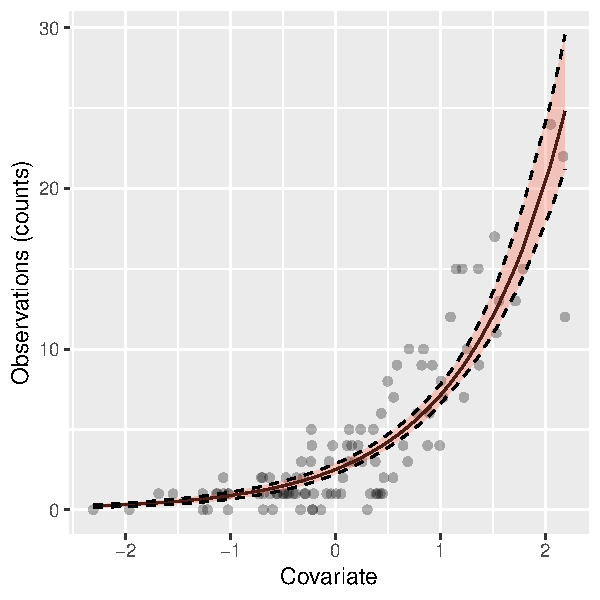
\includegraphics{GLM_ex_files/figure-pdf/unnamed-chunk-7-1.pdf}

}

\caption{Data and 95\% credible intervals}

\end{figure}%

\subsection{R Code}

\begin{Shaded}
\begin{Highlighting}[]
\NormalTok{pred\_glm }\SpecialCharTok{\%\textgreater{}\%} \FunctionTok{ggplot}\NormalTok{() }\SpecialCharTok{+} 
  \FunctionTok{geom\_point}\NormalTok{(}\FunctionTok{aes}\NormalTok{(x,y), }\AttributeTok{alpha =} \FloatTok{0.3}\NormalTok{) }\SpecialCharTok{+}
  \FunctionTok{geom\_line}\NormalTok{(}\FunctionTok{aes}\NormalTok{(x,mean)) }\SpecialCharTok{+}
    \FunctionTok{geom\_ribbon}\NormalTok{(}\FunctionTok{aes}\NormalTok{(}\AttributeTok{x =}\NormalTok{ x, }\AttributeTok{ymax =}\NormalTok{ q0}\FloatTok{.975}\NormalTok{, }\AttributeTok{ymin =}\NormalTok{ q0}\FloatTok{.025}\NormalTok{),}\AttributeTok{fill =} \StringTok{"tomato"}\NormalTok{, }\AttributeTok{alpha =} \FloatTok{0.3}\NormalTok{)}\SpecialCharTok{+}
  \FunctionTok{xlab}\NormalTok{(}\StringTok{"Covariate"}\NormalTok{) }\SpecialCharTok{+} \FunctionTok{ylab}\NormalTok{(}\StringTok{"Observations (counts)"}\NormalTok{)}
\end{Highlighting}
\end{Shaded}

::: \{.callout-warning icon=``false''\} \#\# Task

Suppose a binary response such that

\[
\begin{aligned}
y_i &\sim \mathrm{Bernoulli}(\psi_i)\\
\eta_i &= \mathrm{logit}(\psi_i) = \alpha_0 +\alpha_1 \times w_i 
\end{aligned}
\] Using the following simulated data, use \texttt{inlabru}to fit the
logistic regression above. Then, plot the predictions for 10 new
observations.

\begin{Shaded}
\begin{Highlighting}[]
\FunctionTok{set.seed}\NormalTok{(}\DecValTok{123}\NormalTok{)}
\NormalTok{n }\OtherTok{=} \DecValTok{100}
\NormalTok{alpha }\OtherTok{=} \FunctionTok{c}\NormalTok{(}\FloatTok{0.5}\NormalTok{,}\FloatTok{1.5}\NormalTok{)}
\NormalTok{w }\OtherTok{=} \FunctionTok{rnorm}\NormalTok{(n)}
\NormalTok{psi }\OtherTok{=} \FunctionTok{plogis}\NormalTok{(alpha[}\DecValTok{1}\NormalTok{] }\SpecialCharTok{+}\NormalTok{ alpha[}\DecValTok{2}\NormalTok{] }\SpecialCharTok{*}\NormalTok{ w)}
\NormalTok{y }\OtherTok{=} \FunctionTok{rbinom}\NormalTok{(}\AttributeTok{n =}\NormalTok{ n, }\AttributeTok{size =} \DecValTok{1}\NormalTok{, }\AttributeTok{prob =}\NormalTok{  psi) }\CommentTok{\# set size = 1 to draw binary observations}
\NormalTok{df\_logis }\OtherTok{=} \FunctionTok{data.frame}\NormalTok{(}\AttributeTok{y =}\NormalTok{ y, }\AttributeTok{w =}\NormalTok{ w)  }
\end{Highlighting}
\end{Shaded}

Here we use the logit link function
\(\mathrm{logit}(x) = \log\left(\frac{x}{1-x}\right)\)
(\texttt{plogis()} function in R) to link the linear predictor to the
probabilities \(\psi\).

Take hint

You can set \texttt{family\ =\ "binomial"} for binary responses and the
\(plogis()\) function for computing the predicts probabilities at new
observations.

\begin{tcolorbox}[enhanced jigsaw, toptitle=1mm, bottomrule=.15mm, rightrule=.15mm, colframe=quarto-callout-note-color-frame, colback=white, toprule=.15mm, opacitybacktitle=0.6, titlerule=0mm, bottomtitle=1mm, title=\textcolor{quarto-callout-note-color}{\faInfo}\hspace{0.5em}{Note}, left=2mm, arc=.35mm, leftrule=.75mm, colbacktitle=quarto-callout-note-color!10!white, opacityback=0, coltitle=black, breakable]

The default distribution is \(\mathrm{Binomial}(1, \psi)\). However, if
you have proportional data
(e.g.~\(\dfrac{\mathrm{no.~successes}}{\mathrm{no.~of~  trials}}\)) you
can specify the number of events as your response and then the number of
trials via the \(Ntrials = n\) option in the \texttt{bru\_obs}function.

\end{tcolorbox}

Click here to see the solution

\begin{Shaded}
\begin{Highlighting}[]
\CommentTok{\# Model components}
\NormalTok{cmp\_logis }\OtherTok{=}  \ErrorTok{\textasciitilde{}} \FunctionTok{Intercept}\NormalTok{(}\DecValTok{1}\NormalTok{) }\SpecialCharTok{+} \FunctionTok{w\_effect}\NormalTok{(w, }\AttributeTok{model =} \StringTok{"linear"}\NormalTok{)}
\CommentTok{\# Model likelihood}
\NormalTok{lik\_logis }\OtherTok{=}  \FunctionTok{bru\_obs}\NormalTok{(}\AttributeTok{formula =}\NormalTok{ y }\SpecialCharTok{\textasciitilde{}}\NormalTok{.,}
            \AttributeTok{family =} \StringTok{"binomial"}\NormalTok{,}
            \AttributeTok{data =}\NormalTok{ df\_logis)}
\CommentTok{\# fit the model}
\NormalTok{fit\_logis }\OtherTok{\textless{}{-}} \FunctionTok{bru}\NormalTok{(cmp\_logis,lik\_logis)}

\CommentTok{\# Define data for prediction}
\NormalTok{new\_data }\OtherTok{=} \FunctionTok{data.frame}\NormalTok{(}\AttributeTok{w =} \FunctionTok{c}\NormalTok{(df\_logis}\SpecialCharTok{$}\NormalTok{w, }\FunctionTok{runif}\NormalTok{(}\DecValTok{10}\NormalTok{)),}
                      \AttributeTok{y =} \FunctionTok{c}\NormalTok{(df\_logis}\SpecialCharTok{$}\NormalTok{y, }\FunctionTok{rep}\NormalTok{(}\ConstantTok{NA}\NormalTok{,}\DecValTok{10}\NormalTok{)))}
\CommentTok{\# Define predictor formula}
\NormalTok{pred\_fml }\OtherTok{\textless{}{-}} \ErrorTok{\textasciitilde{}} \FunctionTok{plogis}\NormalTok{(Intercept }\SpecialCharTok{+}\NormalTok{ w\_effect)}

\CommentTok{\# Generate predictions}
\NormalTok{pred\_logis }\OtherTok{\textless{}{-}} \FunctionTok{predict}\NormalTok{(fit\_logis, new\_data, pred\_fml)}

\CommentTok{\# Plot predictions}
\NormalTok{pred\_logis }\SpecialCharTok{\%\textgreater{}\%} \FunctionTok{ggplot}\NormalTok{() }\SpecialCharTok{+} 
  \FunctionTok{geom\_point}\NormalTok{(}\FunctionTok{aes}\NormalTok{(w,y), }\AttributeTok{alpha =} \FloatTok{0.3}\NormalTok{) }\SpecialCharTok{+}
  \FunctionTok{geom\_line}\NormalTok{(}\FunctionTok{aes}\NormalTok{(w,mean)) }\SpecialCharTok{+}
    \FunctionTok{geom\_ribbon}\NormalTok{(}\FunctionTok{aes}\NormalTok{(}\AttributeTok{x =}\NormalTok{ w, }\AttributeTok{ymax =}\NormalTok{ q0}\FloatTok{.975}\NormalTok{, }\AttributeTok{ymin =}\NormalTok{ q0}\FloatTok{.025}\NormalTok{),}\AttributeTok{fill =} \StringTok{"tomato"}\NormalTok{, }\AttributeTok{alpha =} \FloatTok{0.3}\NormalTok{)}\SpecialCharTok{+}
  \FunctionTok{xlab}\NormalTok{(}\StringTok{"Covariate"}\NormalTok{) }\SpecialCharTok{+} \FunctionTok{ylab}\NormalTok{(}\StringTok{"Observations"}\NormalTok{)}
\end{Highlighting}
\end{Shaded}

\begin{verbatim}
Warning: Removed 10 rows containing missing values or values outside the scale range
(`geom_point()`).
\end{verbatim}

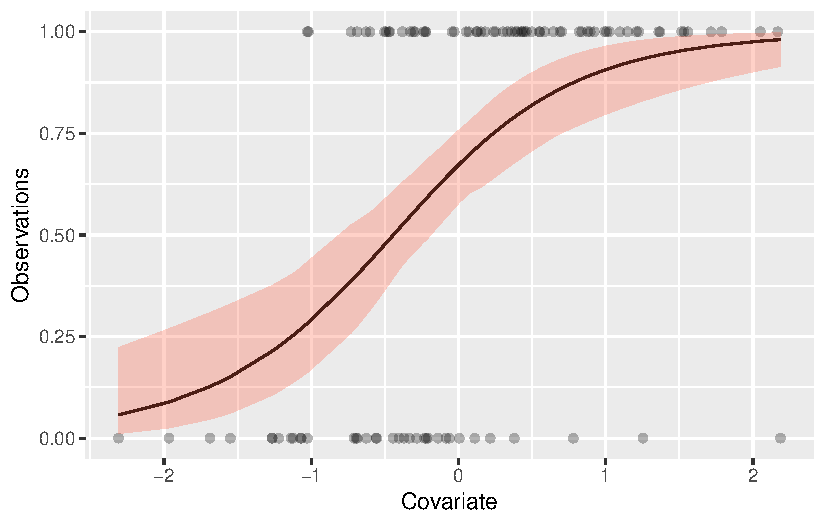
\includegraphics{GLM_ex_files/figure-pdf/unnamed-chunk-10-1.pdf}

:::



\end{document}
